
            \documentclass[tikz]{standalone}
            \begin{document}
            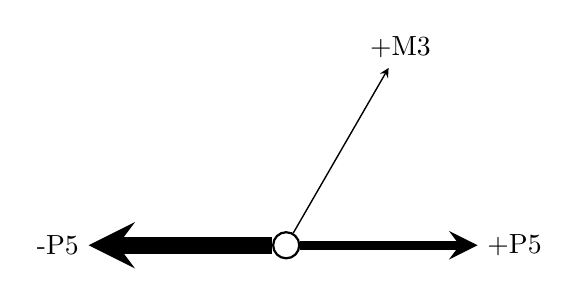
\begin{tikzpicture}[scale=3.5, ->, >=stealth]

            % the circle
            \node (origin) at (0,0) [draw,circle,black,fill=white,thick]{};
            % constant scaling for widths
            \def\cons{10}
            
                    \node (0) at +(0*360/6:0.8286002044123932) {+P5};
                    \path (origin) edge [line width=\cons*0.3421026882919327] node {} (0);
                    
                    \node (3) at +(-3*360/6:0.8286002044123932) {-P5};
                    \path (origin) edge [line width=\cons*0.6074335666622802] node {} (3);
                    
                    \node (5) at +(-5*360/6:0.8286002044123932) {+M3};
                    \path (origin) edge [line width=\cons*0.05046374504578738] node {} (5);
                    
            \end{tikzpicture}
            \end{document}
            